% ============================================================
% Software Requirements Specification (SRS) - SkillSim
% Based on the IEEE 29148 SRS template.
%
% Compile with pdflatex (recommended: Overleaf - upload this single
% file, no external images required, all diagrams are native TikZ).
% Run pdflatex twice (or let Overleaf auto-recompile) so the table
% of contents resolves.
%
% EDIT ME: author names / institution in the \author{} block below.
% ============================================================
\documentclass[11pt]{article}

\usepackage[margin=0.9in]{geometry}
\usepackage{amsmath,amssymb}
\usepackage{booktabs}
\usepackage{longtable}
\usepackage{array}
\usepackage{enumitem}
\usepackage{xcolor}
\usepackage{tikz}
\usetikzlibrary{arrows.meta,positioning,shapes.geometric,shapes.multipart,calc,fit,backgrounds}
\usepackage[colorlinks=true,linkcolor=blue!50!black,urlcolor=blue!50!black,citecolor=blue!50!black]{hyperref}
\usepackage{titlesec}
\usepackage{fancyhdr}

\setlist{noitemsep, topsep=2pt, parsep=0pt, partopsep=0pt}

\pagestyle{fancy}
\fancyhf{}
\fancyhead[L]{SkillSim -- Software Requirements Specification}
\fancyhead[R]{\thepage}
\renewcommand{\headrulewidth}{0.4pt}

% Compact "requirement card" macro, used in Sections 3 and 9.
\newcommand{\frcard}[8]{%
  \par\noindent
  \begin{tabular}{@{}p{0.97\linewidth}@{}}
  \small
  \textbf{Requirement ID:} #1 \quad\textbf{Title:} #2\\[2pt]
  \textbf{Description:} #3\\[2pt]
  \textbf{Inputs:} #4\\[2pt]
  \textbf{Processing:} #5\\[2pt]
  \textbf{Outputs:} #6\\[2pt]
  \textbf{Priority:} #7\\[2pt]
  \textbf{Acceptance Criteria:} #8
  \end{tabular}
  \par\vspace{4mm}
}

\title{\vspace{-1.5cm}Software Requirements Specification\\[2pt]
\Large SkillSim -- A Browser-Based Hands-On Lab Learning Platform\\[4pt]
\normalsize (IEEE 29148 Based)}
% EDIT ME: replace with your real names / institution / course
\author{Vivek Reddy and Team SkillSim \\
\small Department of Computer Science, [University Name], [Course Name / Number] \\
\small vivekreddy9036@gmail.com}
\date{Version 1.1 \quad -- \quad September 17, 2026}

\begin{document}
\maketitle
\thispagestyle{empty}

\begin{abstract}
\noindent This Software Requirements Specification (SRS) describes
SkillSim, a browser-based, hands-on lab platform modeled on the
KodeKloud learning experience. Students work through auto-validated,
step-by-step labs inside real, ephemeral sandbox containers reached
through an in-browser terminal, with each step's completion verified
by executing a validation script inside the student's own container
rather than by self-report. This document follows the IEEE 29148 SRS
structure and covers scope, functional and non-functional
requirements, interfaces, data model, use cases, analysis models,
security requirements, risk analysis, a STRIDE threat model and
OWASP Top 10 vulnerability mapping, software security economics,
security test cases, a requirement traceability matrix, and
acceptance criteria for the project's five-week, single-VM,
no-Kubernetes release.
\end{abstract}

\newpage
\tableofcontents
\newpage

% ============================================================
\section{Introduction}

\subsection{Purpose}
This SRS defines the functional and non-functional requirements of
SkillSim, a hands-on labs platform for technical skill practice. It
guides implementation, serves as a contract between the project team
and course stakeholders, and is a durable reference for extending the
system beyond its initial five-week scope.

\subsection{Scope}
SkillSim lets a student browse a catalog of technology \emph{tracks}
(e.g., Docker, Linux), select a \emph{lab} within a track, and work
through an ordered sequence of \emph{steps} inside a real, ephemeral
sandbox container reachable through an in-browser terminal. Each step
ships with a validation script; when a student believes a step is
complete, the platform executes that script inside the student's live
container and automatically unlocks the next step only on success.
Progress and points are persisted per user. The initial release
targets a single host VM, a hand-authored (non-CMS) content pipeline,
and excludes Kubernetes-based orchestration, multi-node scaling, and
third-party LMS integration.

\subsection{Definitions, Acronyms and Abbreviations}
\begin{itemize}
\item \textbf{Track} -- A named grouping of related labs (e.g., "Docker").
\item \textbf{Lab} -- A single hands-on exercise composed of ordered steps.
\item \textbf{Step} -- One unit of instruction within a lab, paired with
      a validation script.
\item \textbf{Sandbox} -- An ephemeral, hardened Docker container spawned
      for one user's lab session.
\item \textbf{JWT} -- JSON Web Token; a short-lived,
      \texttt{sandbox:attach}-scoped credential authorizing a WebSocket
      terminal connection to one specific session.
\item \textbf{DinD} -- Docker-in-Docker; a sandbox running its own
      nested Docker daemon, used only by labs that teach Docker itself.
\item \textbf{app-backend} -- The REST/database-owning service.
\item \textbf{terminal-server} -- The service that owns the Docker
      socket and bridges WebSocket terminal I/O.
\item \textbf{RTM} -- Requirement Traceability Matrix.
\end{itemize}

\subsection{References}
\begin{enumerate}
\item ISO/IEC/IEEE 29148:2018, \emph{Systems and software engineering
      -- Life cycle processes -- Requirements engineering}.
\item IEEE Std 830-1998, \emph{IEEE Recommended Practice for Software
      Requirements Specifications}.
\item Docker Inc., \emph{Docker Engine API Reference}, docs.docker.com.
\item KodeKloud, \emph{Hands-on Labs Platform} (UX reference),
      kodekloud.com.
\item Prisma Data Platform, \emph{Prisma ORM Documentation},
      prisma.io/docs.
\item OWASP Foundation, \emph{OWASP Top Ten}, owasp.org.
\end{enumerate}

\subsection{Document Overview}
Section 2 describes the product at a high level. Section 3 lists
functional requirements as individual cards. Section 4 covers
non-functional requirements. Section 5 defines external interfaces.
Section 6 defines the data model. Section 7 specifies use cases.
Section 8 presents five analysis-model diagrams. Section 9 details
security requirements. Section 10 is a risk analysis. Section 11 maps
the project's four course outcomes (CO1--CO4) to concrete
threat-modeling, security-economics, and security-testing
deliverables. Section 12 is the requirement traceability matrix.
Section 13 gives measurable acceptance criteria. Section 14 contains
appendices.

% ============================================================
\section{Overall Description}

\subsection{Product Perspective}
SkillSim is a new, self-contained system. It is composed of three
deployable units sharing one host VM during the class-project phase:
a single-page \emph{frontend}, a REST \emph{app-backend} that owns the
relational database, and a \emph{terminal-server} that exclusively
owns the Docker socket and all container lifecycle operations. This
separation confines privileged Docker access to one process, so a
compromised or buggy REST endpoint cannot directly manipulate
containers.

\subsection{Product Functions}
\begin{itemize}
\item Register, authenticate, and browse a catalog of tracks and labs.
\item Start a lab session, provisioning an ephemeral sandbox container
      scoped to that session.
\item Provide an interactive terminal into the sandbox over WebSocket.
\item Present step-by-step lesson content beside the terminal.
\item Auto-validate each step by executing a validation script inside
      the student's own container, unlocking the next step only on
      success.
\item Persist per-user progress and award points on success.
\item Let content authors publish labs as plain files, without a CMS.
\end{itemize}

\subsection{User Classes and Characteristics}
\begin{itemize}
\item \textbf{Student (primary actor):} Browser only; basic
      command-line familiarity assumed.
\item \textbf{Content Author (project team):} Authors labs as files
      under \texttt{labs/\textless track\textgreater/\textless
      lab-slug\textgreater/} and runs a sync script; needs git/shell
      access, not a special UI.
\item \textbf{System actor -- terminal-server:} Not human; spawns,
      execs into, and reaps sandbox containers on students' behalf.
\end{itemize}

\subsection{Operating Environment}
A single Linux VM with a working Docker Engine installation. The
app-backend and terminal-server are Node.js/TypeScript services;
persistent state lives in PostgreSQL. The frontend is a static SPA
(Vite/React) served to any evergreen desktop browser with WebSocket
support. No Kubernetes or multi-host scheduling is in scope.

\subsection{Design and Implementation Constraints}
\begin{itemize}
\item \textbf{Timeline:} Five-week class-project schedule; scope is
      fixed, not expanded mid-project.
\item \textbf{Single VM:} All services and the database co-locate on
      one host.
\item \textbf{No Kubernetes:} Sandboxes are scheduled directly against
      the local Docker Engine.
\item \textbf{File-based content only:} No admin UI/CMS for authoring
      labs.
\item \textbf{Auto-validation only:} Steps advance strictly via a
      passing validation script -- manual "mark as done" is out of
      scope.
\end{itemize}

\subsection{Assumptions and Dependencies}
The host VM has sufficient CPU/memory to run several concurrent
ephemeral containers; Docker images for each lab are pre-built and
tagged before publishing; students have a modern browser. The system
depends on the Docker Engine API, PostgreSQL, and standard JWT
libraries; no third-party SaaS dependency is required at runtime.

% ============================================================
\section{Functional Requirements}
Each requirement below follows the ID / Title / Description / Inputs
/ Processing / Outputs / Priority / Acceptance Criteria format.
Priority uses MoSCoW (Must/Should/Could).

\frcard{FR-01}{User Registration}
 {The system shall allow a new user to register with an email,
 password, and display name.}
 {Email, password, display name.}
 {Validate email format and uniqueness; hash password; create
 \texttt{User} row.}
 {Created user account; redirect to catalog.}
 {Must}
 {A new, unique email registers successfully in under 2 seconds; a
 duplicate email is rejected with a clear error.}

\frcard{FR-02}{User Login}
 {The system shall authenticate registered users using email and
 password.}
 {Email, password.}
 {Look up user by email; verify password hash; issue session
 credential.}
 {Authenticated session; user redirected to dashboard/catalog.}
 {Must}
 {Valid users are authenticated within 2 seconds; invalid credentials
 are rejected without revealing which field was wrong.}

\frcard{FR-03}{Browse Tracks and Labs}
 {The system shall list all tracks and, per track, the labs it
 contains, including title, difficulty, and duration.}
 {Track slug (optional, for detail view).}
 {Query \texttt{Track} and related \texttt{Lab} rows ordered by
 \texttt{orderInTrack}.}
 {Rendered catalog / track-detail page.}
 {Must}
 {Catalog page loads all tracks in under 1 second on the reference
 dataset; track detail lists labs in the authored order.}

\frcard{FR-04}{Start Lab Session}
 {The system shall provision an ephemeral sandbox container from the
 lab's pre-built image and issue a session-scoped JWT when a student
 starts a lab.}
 {User ID (from session), lab slug.}
 {Create \texttt{UserLabSession} row; embed step validation-script
 filenames in JWT claims; request container spawn.}
 {Sandbox JWT (\texttt{sandbox:attach} scope); active session record.}
 {Must}
 {A lab start results in a running container and a valid JWT within a
 few seconds; the JWT is rejected if reused for a different session.}

\frcard{FR-05}{Interactive Terminal Session}
 {The system shall open an interactive terminal into the student's
 sandbox over WebSocket, verifying the JWT and request Origin before
 upgrade.}
 {Sandbox JWT, WebSocket upgrade request, keystrokes, resize events.}
 {Verify JWT + Origin; \texttt{docker exec} with \texttt{Tty:true};
 bridge binary frames bidirectionally.}
 {Live terminal I/O; resized PTY on window resize.}
 {Must}
 {A valid JWT opens a working shell within 2 seconds; an invalid or
 expired JWT is rejected before any container access occurs.}

\frcard{FR-06}{Check Step (Auto-Validation)}
 {The system shall execute the current step's validation script inside
 the student's own container when the student triggers a Check action,
 and report pass/fail.}
 {\texttt{check\_step} control frame identifying the current step.}
 {Exec the step's \texttt{.check.sh} script inside the session's
 container; capture exit code.}
 {\texttt{step\_result:\{passed:boolean\}} sent back over the
 WebSocket.}
 {Must}
 {A correctly completed step returns \texttt{passed:true}; an
 incomplete step returns \texttt{passed:false} without crashing the
 session.}

\frcard{FR-07}{Unlock Next Step and Award Points}
 {The system shall unlock the next step and award points only after
 the current step's validation script reports success.}
 {Passing \texttt{step\_result} from FR-06.}
 {terminal-server calls \texttt{/internal/progress}; app-backend
 updates \texttt{UserStepProgress.status} and \texttt{User.points}.}
 {Persisted progress row; updated point total; unlocked next step in
 the UI.}
 {Must}
 {After a passing check, \texttt{UserStepProgress.status=completed}
 and the point increment are visible in the database and reflected in
 the UI without a page reload.}

\frcard{FR-08}{Idle Session Reaping}
 {The system shall idle-reap sandbox containers and mark sessions
 expired after a period of client inactivity.}
 {Session last-activity timestamp.}
 {Background sweep compares last activity to an idle threshold;
 removes container; updates session status.}
 {Freed host resources; \texttt{UserLabSession.status=expired}.}
 {Should}
 {A session with no WebSocket activity beyond the configured threshold
 has its container removed and status updated without manual
 intervention.}

\frcard{FR-09}{Author and Publish Lab Content}
 {The system shall let a content author publish a new lab by adding
 files under \texttt{labs/\textless track\textgreater/} and running a
 sync script, without application code changes.}
 {\texttt{lab.yaml}, step Markdown files, \texttt{*.check.sh} scripts.}
 {\texttt{scripts/sync-labs.ts} parses lab content and upserts
 \texttt{Track}/\texttt{Lab}/\texttt{LabStep} rows via Prisma.}
 {New or updated catalog entries visible to students.}
 {Must}
 {A new, correctly formatted lab directory appears in the catalog
 after running the sync script, with no code deployment required.}

\frcard{FR-10}{Privileged (DinD) Sandbox Support}
 {The system shall support a distinct, narrower-trust "privileged"
 container profile for labs that require a nested Docker daemon.}
 {\texttt{Lab.privileged} flag.}
 {terminal-server branches container-spawn options to grant the
 minimum additional privilege needed for nested Docker, without
 mounting the host socket.}
 {A working nested Docker daemon inside an otherwise ephemeral,
 resource-capped container.}
 {Should}
 {A DinD lab's steps (e.g., \texttt{docker run} inside the sandbox)
 complete successfully; the host Docker socket is never reachable from
 inside the sandbox.}

\frcard{FR-11}{Student Dashboard}
 {The system shall display a dashboard summarizing a student's total
 points and completed labs.}
 {User ID (from session).}
 {Aggregate \texttt{UserStepProgress} and \texttt{User.points} for the
 current user.}
 {Rendered dashboard view.}
 {Could}
 {Dashboard totals match the sum of completed, points-bearing steps in
 the database for that user.}

\frcard{FR-12}{Session Result Reporting (Internal)}
 {The system shall accept step-result reports only from
 terminal-server, authenticated by a shared secret, on a dedicated
 internal endpoint.}
 {Shared secret header, session ID, step ID, pass/fail.}
 {Verify shared secret; write \texttt{UserStepProgress}; award
 points.}
 {200 OK with updated progress, or 401 if the secret is missing/wrong.}
 {Must}
 {Calls without the correct shared secret are rejected; calls with it
 persist progress exactly once per (session, step) pair.}

% ============================================================
\section{Non-Functional Requirements}

\subsection{Performance}
Terminal keystroke round-trip latency shall remain low enough for
interactive use (target: under 150\,ms end-to-end on a local/LAN
deployment). Step validation shall complete and report a result within
a few seconds for validation scripts of the size used in this
project's labs. The catalog page shall load in under 1 second under
nominal load.

\subsection{Security}
All Docker socket access shall be confined to terminal-server. Full
requirements are detailed in Section 9.

\subsection{Reliability}
Loss of a single sandbox container shall not corrupt persisted
progress, since progress is written only after an explicit, successful
validation report. A terminal-server restart shall not corrupt
app-backend's stored state.

\subsection{Availability}
Within the single-VM class-project scope, the system targets
best-effort availability during scheduled class/demo hours; no formal
uptime SLA applies. Session state is recoverable from PostgreSQL after
a service restart.

\subsection{Usability}
The lab page layout (terminal left, instructions and Check action
right) shall require no explanation for a student already familiar
with common hands-on-lab platforms such as KodeKloud.

\subsection{Maintainability}
Lab content shall be addable or editable purely as version-controlled
files (\texttt{lab.yaml}, step Markdown, \texttt{*.check.sh}), without
modifying application code, so content and platform code evolve
independently.

\subsection{Portability}
The frontend shall run unmodified on any evergreen Chromium-, Gecko-,
or WebKit-based desktop browser with WebSocket support. Backend
services target any Linux host with Docker Engine and PostgreSQL
available, without OS-specific code paths.

% ============================================================
\section{External Interface Requirements}

\subsection{User Interface}
A responsive web UI providing: a catalog page (tracks and labs), a
track detail page, a split-pane lab page (terminal left; Markdown step
panel and Check button right), and a dashboard. All interaction is
through a standard browser; no native client is required.

\subsection{Hardware Interface}
None directly; the system relies on the host VM's CPU, memory, and
container runtime. No specialized hardware is required.

\subsection{Software Interface}
\begin{itemize}
\item \textbf{app-backend REST API:} \texttt{/auth} (signup, login),
      \texttt{/tracks}, \texttt{/tracks/:slug}, \texttt{/labs/:slug},
      \texttt{/labs/:slug/start}, \texttt{/internal/progress}
      (shared-secret protected).
\item \textbf{terminal-server WebSocket API:} \texttt{/term} upgrade
      endpoint carrying binary terminal frames plus JSON control
      frames (\texttt{resize}, \texttt{check\_step}).
\item \textbf{Docker Engine API:} consumed via \texttt{dockerode} for
      container spawn, exec, and teardown.
\item \textbf{PostgreSQL:} accessed exclusively by app-backend through
      Prisma ORM.
\end{itemize}

\subsection{Communication Interface}
REST calls use HTTPS/JSON in a production deployment; the terminal
uses one persistent WebSocket per active session, carrying both binary
I/O and JSON control messages.

% ============================================================
\section{Data Requirements}

\subsection{Entities}
\texttt{User}, \texttt{Track}, \texttt{Lab}, \texttt{LabStep},
\texttt{UserLabSession}, \texttt{UserStepProgress}.

\subsection{Attributes}
\begin{itemize}
\item \textbf{User}: id, email (unique), passwordHash, displayName,
      points, createdAt.
\item \textbf{Track}: id, slug (unique), name, description, icon.
\item \textbf{Lab}: id, trackId (FK), slug (unique), title,
      description, difficulty, durationMinutes, tags, orderInTrack,
      imageRef, privileged.
\item \textbf{LabStep}: id, labId (FK), stepNumber, title,
      contentMarkdown, validationScript.
\item \textbf{UserLabSession}: id, userId (FK), labId (FK),
      containerId, status, startedAt, endedAt.
\item \textbf{UserStepProgress}: id, sessionId (FK), stepId (FK),
      status, completedAt.
\end{itemize}

\subsection{Relationships}
\begin{itemize}
\item Track (1) -- (\,*\,) Lab
\item Lab (1) -- (\,*\,) LabStep
\item User (1) -- (\,*\,) UserLabSession
\item Lab (1) -- (\,*\,) UserLabSession
\item UserLabSession (1) -- (\,*\,) UserStepProgress
\item LabStep (1) -- (\,*\,) UserStepProgress
\end{itemize}

\subsection{Validation Rules}
\begin{itemize}
\item \texttt{User.email} must be unique and a syntactically valid
      email address.
\item \texttt{Track.slug} and \texttt{Lab.slug} must be unique,
      URL-safe strings.
\item (\texttt{Lab.trackId}, \texttt{Lab.orderInTrack}) should not
      collide within a track (enforced at content-authoring time via
      the sync script).
\item (\texttt{LabStep.labId}, \texttt{LabStep.stepNumber}) must be
      unique -- enforced by a database composite unique constraint.
\item (\texttt{UserStepProgress.sessionId}, \texttt{...stepId}) must
      be unique -- enforced by a database composite unique constraint,
      preventing duplicate progress rows for the same step.
\item \texttt{Lab.difficulty} must be one of \{beginner,
      intermediate, advanced\}; \texttt{UserLabSession.status} must be
      one of \{running, completed, expired, terminated\};
      \texttt{UserStepProgress.status} must be one of \{pending,
      completed\} -- enforced via database enum types.
\end{itemize}

\subsection{Database Requirements}
PostgreSQL is the system of record, accessed exclusively by
app-backend through Prisma ORM, which also manages schema migrations.
Foreign keys enforce referential integrity across all relationships
above; composite unique indexes back the validation rules listed. An
index on (\texttt{trackId}, \texttt{orderInTrack}) supports ordered
lab listing per track, and an index on (\texttt{userId},
\texttt{labId}) supports fast session lookups.

% ============================================================
\section{Use Cases}

\subsubsection*{UC-01: User Registration}
\textbf{Actor(s):} Student.\\
\textbf{Preconditions:} Actor has a valid, unregistered email address.\\
\textbf{Main Flow:}
\begin{enumerate}
\item Actor submits email, password, and display name.
\item System validates the email format and checks uniqueness.
\item System hashes the password and creates a \texttt{User} record.
\item System returns an authenticated session and redirects to the
      catalog.
\end{enumerate}
\textbf{Alternate Flow:} If the email is already registered, the
system rejects the request with a clear, non-account-enumerating
error and the actor may retry with different credentials.\\
\textbf{Postconditions:} A new \texttt{User} row exists; the actor is
authenticated.

\subsubsection*{UC-02: User Login}
\textbf{Actor(s):} Student.\\
\textbf{Preconditions:} Actor has a registered account.\\
\textbf{Main Flow:}
\begin{enumerate}
\item Actor submits email and password.
\item System looks up the user and verifies the password hash.
\item System issues an authenticated session.
\end{enumerate}
\textbf{Alternate Flow:} If credentials are invalid, the system
returns a generic authentication error without revealing whether the
email exists.\\
\textbf{Postconditions:} Actor holds a valid authenticated session.

\subsubsection*{UC-03: Browse Catalog and Start a Lab}
\textbf{Actor(s):} Student.\\
\textbf{Preconditions:} Actor is authenticated.\\
\textbf{Main Flow:}
\begin{enumerate}
\item Actor views the track catalog and selects a track.
\item System lists that track's labs in authored order.
\item Actor selects a lab and clicks Start.
\item System provisions an ephemeral sandbox container from the lab's
      image and issues a scoped JWT.
\item Frontend opens a WebSocket terminal session using the JWT.
\end{enumerate}
\textbf{Alternate Flow:} If container provisioning fails (e.g., host
resource exhaustion), the system surfaces an error and does not create
a \texttt{UserLabSession} in \texttt{running} state.\\
\textbf{Postconditions:} A running sandbox and an active
\texttt{UserLabSession} exist for the actor.

\subsubsection*{UC-04: Interactive Terminal Session}
\textbf{Actor(s):} Student; terminal-server (system actor).\\
\textbf{Preconditions:} A sandbox JWT has been issued (UC-03).\\
\textbf{Main Flow:}
\begin{enumerate}
\item Frontend opens a WebSocket to \texttt{/term} with the JWT.
\item terminal-server verifies the JWT and request Origin.
\item terminal-server execs an interactive shell in the session's
      container and bridges binary frames both ways.
\item Actor types commands and sees live output.
\end{enumerate}
\textbf{Alternate Flow:} If the JWT is invalid, expired, or the Origin
does not match, the upgrade is rejected before any container access.\\
\textbf{Postconditions:} Actor has a live shell inside their own
sandbox container.

\subsubsection*{UC-05: Check Step (Auto-Validation)}
\textbf{Actor(s):} Student; terminal-server (system actor).\\
\textbf{Preconditions:} Actor has an active terminal session on an
unlocked step.\\
\textbf{Main Flow:}
\begin{enumerate}
\item Actor performs the step's intended actions in the terminal.
\item Actor clicks Check, sending a \texttt{check\_step} frame.
\item terminal-server execs the step's validation script inside the
      container.
\item On success, terminal-server reports the result to app-backend
      via \texttt{/internal/progress}.
\item app-backend persists \texttt{UserStepProgress}, awards points,
      and the next step unlocks in the UI.
\end{enumerate}
\textbf{Alternate Flow:} If the script exits non-zero, the system
returns \texttt{passed:false}; the current step remains locked and the
actor may retry after correcting their work.\\
\textbf{Postconditions:} On success, progress and points are durably
persisted and the next step is unlocked; on failure, no state changes.

\subsubsection*{UC-06: Idle Session Reaping}
\textbf{Actor(s):} terminal-server (system actor).\\
\textbf{Preconditions:} A \texttt{UserLabSession} is in
\texttt{running} status with no recent activity.\\
\textbf{Main Flow:}
\begin{enumerate}
\item A background sweep identifies sessions idle past the configured
      threshold.
\item terminal-server removes the associated sandbox container.
\item terminal-server updates the session's status to
      \texttt{expired}.
\end{enumerate}
\textbf{Alternate Flow:} If container removal fails, the sweep logs
the failure and retries on the next cycle rather than marking the
session expired prematurely.\\
\textbf{Postconditions:} Host resources are freed; the session no
longer accepts terminal input.

% ============================================================
\section{Analysis Models}

\subsection{Use Case Diagram}
\begin{center}
\resizebox{\linewidth}{!}{%
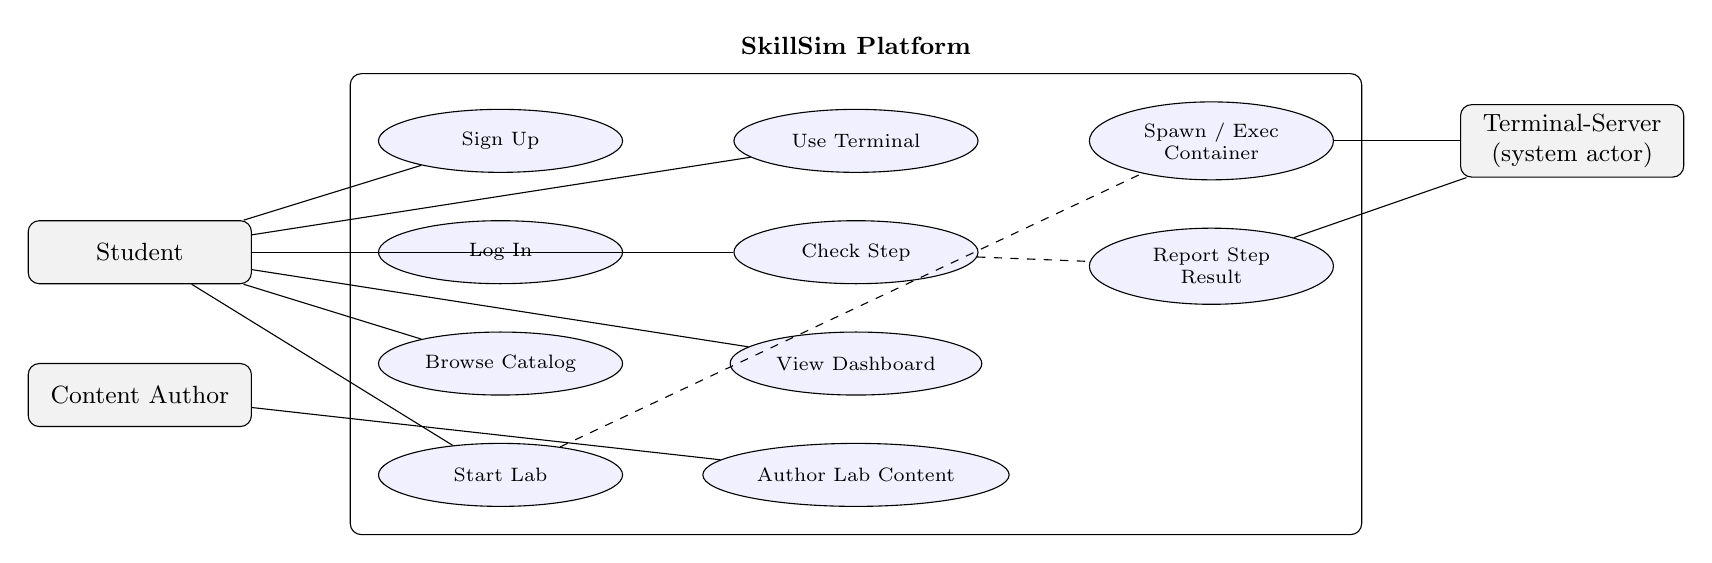
\begin{tikzpicture}[
  actor/.style={rectangle, draw, rounded corners, fill=gray!10,
                align=center, font=\small, minimum height=8mm,
                text width=2.6cm},
  uc/.style={ellipse, draw, fill=blue!6, align=center, font=\scriptsize,
             minimum width=3.1cm, minimum height=8mm},
  sysbound/.style={rectangle, draw, rounded corners, inner sep=10pt}
]
  % use cases
  \node[uc] (uc1) {Sign Up};
  \node[uc, below=6mm of uc1] (uc2) {Log In};
  \node[uc, below=6mm of uc2] (uc3) {Browse Catalog};
  \node[uc, below=6mm of uc3] (uc4) {Start Lab};
  \node[uc, right=14mm of uc1] (uc5) {Use Terminal};
  \node[uc, below=6mm of uc5] (uc6) {Check Step};
  \node[uc, below=6mm of uc6] (uc7) {View Dashboard};
  \node[uc, below=6mm of uc7] (uc8) {Author Lab Content};
  \node[uc, right=14mm of uc5] (uc9) {Spawn / Exec\\Container};
  \node[uc, below=6mm of uc9] (uc10) {Report Step\\Result};

  \begin{scope}[on background layer]
    \node[sysbound, fit=(uc1)(uc4)(uc5)(uc8)(uc9)(uc10)] (bound) {};
  \end{scope}
  \node[font=\bfseries\small] at ($(bound.north)+(0,0.35)$) {SkillSim Platform};

  \node[actor, left=16mm of uc2] (student) {Student};
  \node[actor, below=10mm of student] (author) {Content Author};
  \node[actor, right=16mm of uc9] (tserver) {Terminal-Server\\(system actor)};

  \draw (student) -- (uc1);
  \draw (student) -- (uc2);
  \draw (student) -- (uc3);
  \draw (student) -- (uc4);
  \draw (student) -- (uc5);
  \draw (student) -- (uc6);
  \draw (student) -- (uc7);
  \draw (author) -- (uc8);
  \draw (tserver) -- (uc9);
  \draw (tserver) -- (uc10);
  \draw[dashed] (uc4) -- (uc9);
  \draw[dashed] (uc6) -- (uc10);
\end{tikzpicture}}
\end{center}

\subsection{Activity Diagram}
\begin{center}
\resizebox{0.85\linewidth}{!}{%
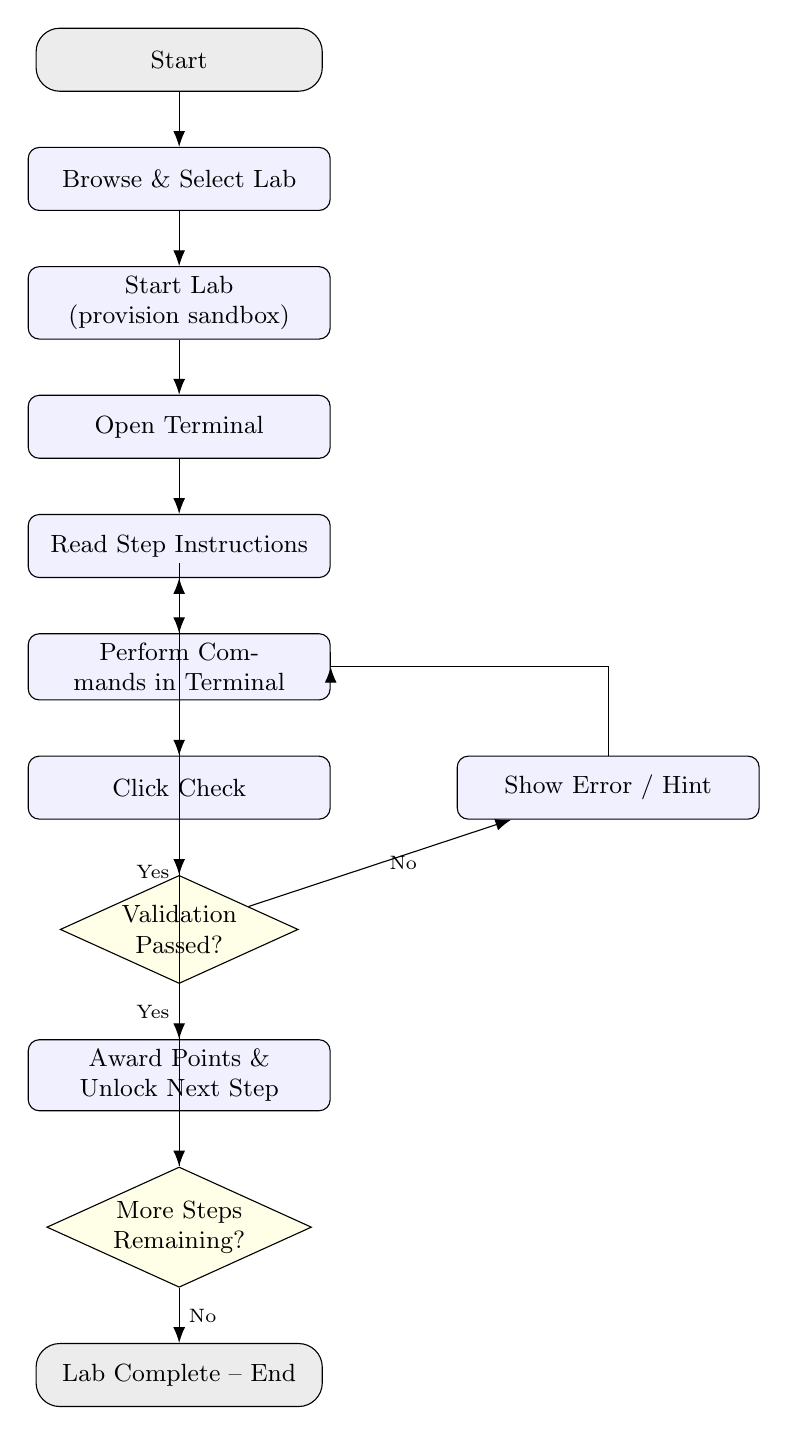
\begin{tikzpicture}[
  node distance=7mm and 10mm,
  start/.style={rounded corners=3mm, draw, fill=gray!15, minimum height=8mm, text width=3.4cm, align=center, font=\small},
  act/.style={rectangle, draw, rounded corners, fill=blue!6, minimum height=8mm, text width=3.6cm, align=center, font=\small},
  dec/.style={diamond, draw, fill=yellow!10, aspect=2.2, inner sep=1pt, font=\small, align=center},
  arr/.style={-{Latex[length=2mm]}}
]
  \node[start] (s0) {Start};
  \node[act, below=of s0] (a1) {Browse \& Select Lab};
  \node[act, below=of a1] (a2) {Start Lab\\(provision sandbox)};
  \node[act, below=of a2] (a3) {Open Terminal};
  \node[act, below=of a3] (a4) {Read Step Instructions};
  \node[act, below=of a4] (a5) {Perform Commands in Terminal};
  \node[act, below=of a5] (a6) {Click Check};
  \node[dec, below=of a6] (d1) {Validation\\Passed?};
  \node[act, right=16mm of a6] (a7) {Show Error / Hint};
  \node[act, below=of d1] (a8) {Award Points \&\\Unlock Next Step};
  \node[dec, below=of a8] (d2) {More Steps\\Remaining?};
  \node[start, below=of d2] (s1) {Lab Complete -- End};

  \draw[arr] (s0) -- (a1);
  \draw[arr] (a1) -- (a2);
  \draw[arr] (a2) -- (a3);
  \draw[arr] (a3) -- (a4);
  \draw[arr] (a4) -- (a5);
  \draw[arr] (a5) -- (a6);
  \draw[arr] (a6) -- (d1);
  \draw[arr] (d1) -- node[right, font=\scriptsize]{No} (a7);
  \draw[arr] (a7.north) |- ($(a5.east)+(0,0)$) -- (a5.east);
  \draw[arr] (d1) -- node[left, font=\scriptsize]{Yes} (a8);
  \draw[arr] (a8) -- (d2);
  \draw[arr] (d2) -- node[left, font=\scriptsize]{Yes} (a4.south -| d2) -- (a4);
  \draw[arr] (d2) -- node[right, font=\scriptsize]{No} (s1);
\end{tikzpicture}}
\end{center}

\subsection{Sequence Diagram}
\emph{Flow: student starts a lab, opens a terminal, and successfully
checks a step.}
\begin{center}
\resizebox{\linewidth}{!}{%
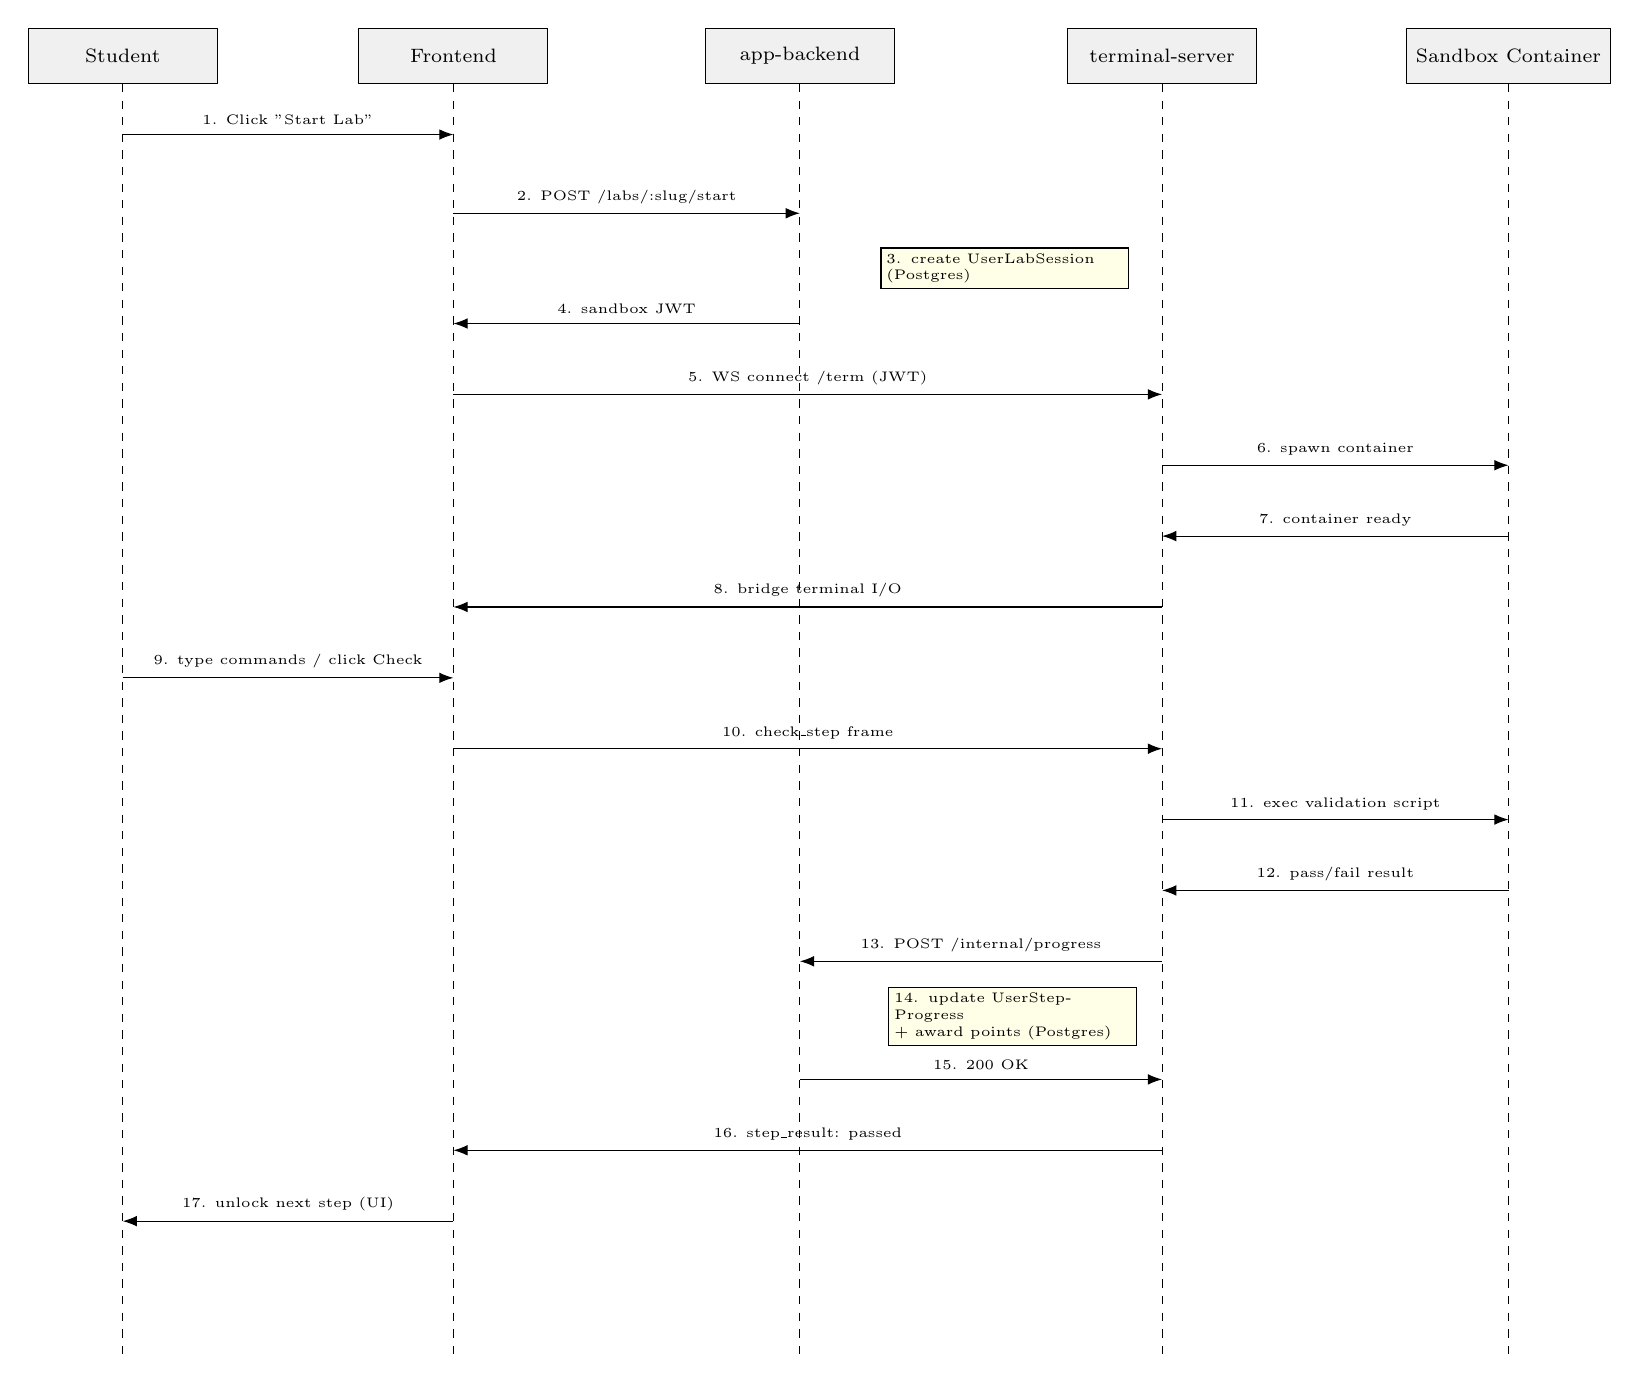
\begin{tikzpicture}[
  lifeline/.style={dashed},
  actorbox/.style={rectangle, draw, fill=gray!12, align=center, font=\scriptsize, minimum width=2.4cm, minimum height=7mm},
  msg/.style={-{Latex[length=1.8mm]}, font=\tiny},
  note/.style={rectangle, draw, fill=yellow!10, font=\tiny, align=left, text width=3.0cm, inner sep=2pt}
]
  \def\sx{0}   \def\fx{4.2} \def\ax{8.6} \def\tx{13.2} \def\cx{17.6}
  \node[actorbox] (S) at (\sx,0) {Student};
  \node[actorbox] (F) at (\fx,0) {Frontend};
  \node[actorbox] (A) at (\ax,0) {app-backend};
  \node[actorbox] (T) at (\tx,0) {terminal-server};
  \node[actorbox] (C) at (\cx,0) {Sandbox Container};

  \draw[lifeline] (S) -- ++(0,-16.5);
  \draw[lifeline] (F) -- ++(0,-16.5);
  \draw[lifeline] (A) -- ++(0,-16.5);
  \draw[lifeline] (T) -- ++(0,-16.5);
  \draw[lifeline] (C) -- ++(0,-16.5);

  \draw[msg] (\sx,-1) -- node[midway,above]{1. Click "Start Lab"} (\fx,-1);
  \draw[msg] (\fx,-2) -- node[midway,above]{2. POST /labs/:slug/start} (\ax,-2);
  \node[note] at (\ax+2.6,-2.7) {3. create UserLabSession (Postgres)};
  \draw[msg] (\ax,-3.4) -- node[midway,above]{4. sandbox JWT} (\fx,-3.4);
  \draw[msg] (\fx,-4.3) -- node[midway,above]{5. WS connect /term (JWT)} (\tx,-4.3);
  \draw[msg] (\tx,-5.2) -- node[midway,above]{6. spawn container} (\cx,-5.2);
  \draw[msg] (\cx,-6.1) -- node[midway,above]{7. container ready} (\tx,-6.1);
  \draw[msg] (\tx,-7.0) -- node[midway,above]{8. bridge terminal I/O} (\fx,-7.0);
  \draw[msg] (\sx,-7.9) -- node[midway,above]{9. type commands / click Check} (\fx,-7.9);
  \draw[msg] (\fx,-8.8) -- node[midway,above]{10. check\_step frame} (\tx,-8.8);
  \draw[msg] (\tx,-9.7) -- node[midway,above]{11. exec validation script} (\cx,-9.7);
  \draw[msg] (\cx,-10.6) -- node[midway,above]{12. pass/fail result} (\tx,-10.6);
  \draw[msg] (\tx,-11.5) -- node[midway,above]{13. POST /internal/progress} (\ax,-11.5);
  \node[note] at (\ax+2.7,-12.2) {14. update UserStepProgress\\+ award points (Postgres)};
  \draw[msg] (\ax,-13.0) -- node[midway,above]{15. 200 OK} (\tx,-13.0);
  \draw[msg] (\tx,-13.9) -- node[midway,above]{16. step\_result: passed} (\fx,-13.9);
  \draw[msg] (\fx,-14.8) -- node[midway,above]{17. unlock next step (UI)} (\sx,-14.8);
\end{tikzpicture}}
\end{center}

\subsection{Class Diagram}
\begin{center}
\resizebox{\linewidth}{!}{%
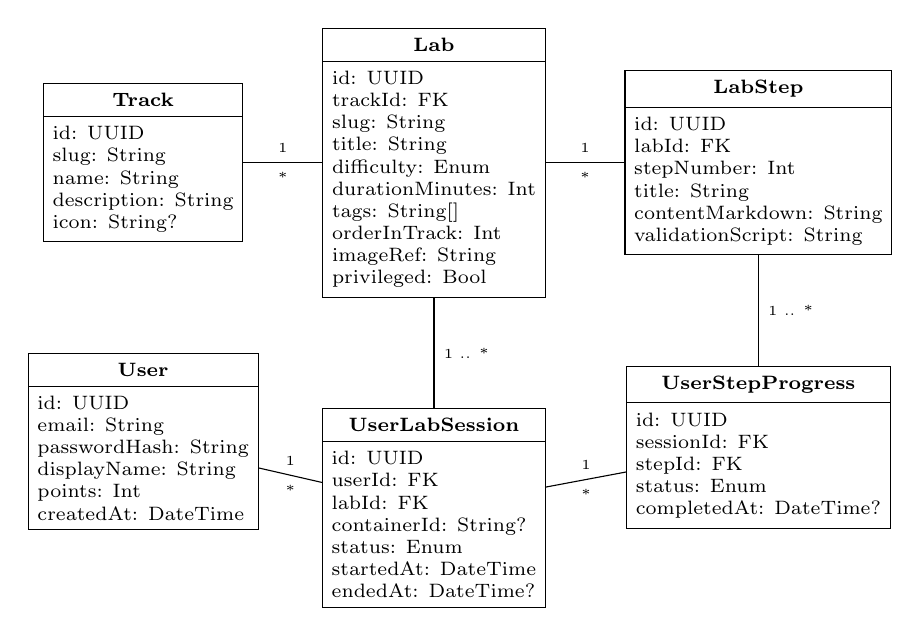
\begin{tikzpicture}[
  cls/.style={rectangle split, rectangle split parts=2, draw,
              font=\scriptsize, align=left, rectangle split part align={center,left}},
  rel/.style={-{}, thin},
  node distance=14mm and 10mm
]
  \node[cls] (Track) {\textbf{Track}
    \nodepart{two} id: UUID\\slug: String\\name: String\\description: String\\icon: String?};
  \node[cls, right=of Track] (Lab) {\textbf{Lab}
    \nodepart{two} id: UUID\\trackId: FK\\slug: String\\title: String\\difficulty: Enum\\durationMinutes: Int\\tags: String[]\\orderInTrack: Int\\imageRef: String\\privileged: Bool};
  \node[cls, right=of Lab] (LabStep) {\textbf{LabStep}
    \nodepart{two} id: UUID\\labId: FK\\stepNumber: Int\\title: String\\contentMarkdown: String\\validationScript: String};

  \node[cls, below=of Track] (User) {\textbf{User}
    \nodepart{two} id: UUID\\email: String\\passwordHash: String\\displayName: String\\points: Int\\createdAt: DateTime};
  \node[cls, below=of Lab] (Session) {\textbf{UserLabSession}
    \nodepart{two} id: UUID\\userId: FK\\labId: FK\\containerId: String?\\status: Enum\\startedAt: DateTime\\endedAt: DateTime?};
  \node[cls, below=of LabStep] (Progress) {\textbf{UserStepProgress}
    \nodepart{two} id: UUID\\sessionId: FK\\stepId: FK\\status: Enum\\completedAt: DateTime?};

  \draw[rel] (Track) -- node[above,font=\tiny]{1} node[below,font=\tiny]{*} (Lab);
  \draw[rel] (Lab) -- node[above,font=\tiny]{1} node[below,font=\tiny]{*} (LabStep);
  \draw[rel] (User) -- node[above,font=\tiny]{1} node[below,font=\tiny]{*} (Session);
  \draw[rel] (Lab) -- node[right,font=\tiny]{1 .. *} (Session);
  \draw[rel] (Session) -- node[above,font=\tiny]{1} node[below,font=\tiny]{*} (Progress);
  \draw[rel] (LabStep) -- node[right,font=\tiny]{1 .. *} (Progress);
\end{tikzpicture}}
\end{center}

\subsection{ER Diagram / Data Model}
\begin{center}
\resizebox{\linewidth}{!}{%
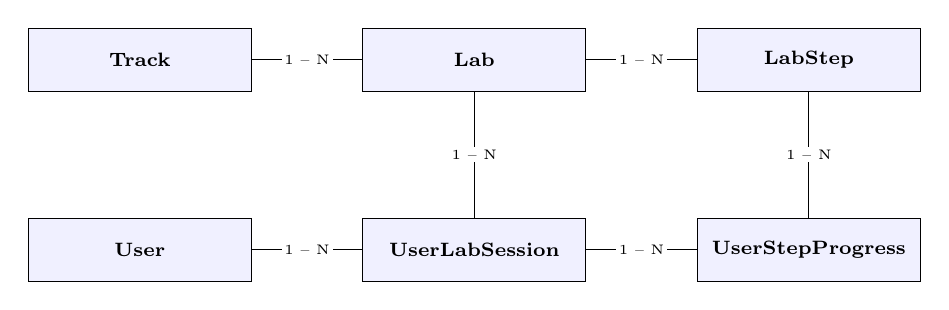
\begin{tikzpicture}[
  ent/.style={rectangle, draw, fill=blue!6, font=\scriptsize\bfseries, minimum height=8mm, text width=2.6cm, align=center},
  rel/.style={-{}, thin},
  lbl/.style={font=\tiny, fill=white, inner sep=1pt},
  node distance=16mm and 14mm
]
  \node[ent] (Track) {Track};
  \node[ent, right=of Track] (Lab) {Lab};
  \node[ent, right=of Lab] (LabStep) {LabStep};
  \node[ent, below=of Track] (User) {User};
  \node[ent, below=of Lab] (Session) {UserLabSession};
  \node[ent, below=of LabStep] (Progress) {UserStepProgress};

  \draw[rel] (Track) -- (Lab) node[lbl, pos=0.5]{1 -- N};
  \draw[rel] (Lab) -- (LabStep) node[lbl, pos=0.5]{1 -- N};
  \draw[rel] (User) -- (Session) node[lbl, pos=0.5]{1 -- N};
  \draw[rel] (Lab) -- (Session) node[lbl, pos=0.5]{1 -- N};
  \draw[rel] (Session) -- (Progress) node[lbl, pos=0.5]{1 -- N};
  \draw[rel] (LabStep) -- (Progress) node[lbl, pos=0.5]{1 -- N};
\end{tikzpicture}}
\end{center}

% ============================================================
\section{Security Requirements}

\subsection{Authentication}
The system shall authenticate students via email and a bcrypt- or
Argon2-hashed password before issuing any session credential.
Sandbox/terminal access shall additionally require a short-lived JWT
scoped to \texttt{sandbox:attach} for one specific session, separate
from the student's login session.

\subsection{Authorization}
A student's JWT shall authorize access only to the sandbox container
of their own active session; terminal-server shall verify the session
ID embedded in the JWT against the requested container before
attaching. The \texttt{/internal/progress} endpoint shall accept
requests only from terminal-server, authenticated by a shared secret
never exposed to the browser.

\subsection{Input Validation}
All REST and WebSocket control-frame inputs shall be validated
server-side (type, length, and allow-listed values) before use,
preventing SQL injection (mitigated structurally by Prisma's
parameterized queries) and cross-site scripting in any rendered
Markdown step content.

\subsection{Encryption}
All communication shall use HTTPS/TLS in a production deployment,
including the WebSocket terminal connection (WSS). Password hashes
shall use bcrypt or Argon2 with a per-user salt; JWTs shall be signed
with a server-held secret not exposed to clients.

\subsection{Logging and Auditing}
The system shall log lab session starts/ends, container spawn/teardown
events, and step check results (pass/fail, timestamp, user, step) to
support debugging and post-hoc auditing of student progress.

\subsection{Session Management}
Sandbox JWTs shall be short-lived and single-session-scoped, rejected
immediately on session expiry, completion, or termination. Idle
sessions shall be reaped per FR-08, releasing both the container and
the session's implicit terminal-access authorization.

\subsection{Backup and Recovery}
PostgreSQL, as the system of record, shall be backed up on a regular
schedule (recommended: nightly logical dump) sufficient to recover
user accounts and progress after host failure. Sandbox containers are
intentionally ephemeral and are not backed up -- only their pass/fail
results, persisted to PostgreSQL, need survive a container's loss.

% ============================================================
\section{Risk Analysis}

\begin{longtable}{@{}p{0.09\linewidth}p{0.34\linewidth}p{0.12\linewidth}p{0.10\linewidth}p{0.30\linewidth}@{}}
\toprule
\textbf{ID} & \textbf{Risk} & \textbf{Likelihood} & \textbf{Impact} & \textbf{Mitigation} \\
\midrule
\endhead
R-01 & Host VM resource exhaustion from too many concurrent sandbox
       containers. & Medium & High & Idle-reap (FR-08) plus a
       per-host concurrency cap on active sessions. \\
R-02 & Docker socket compromise via a terminal-server bug, allowing
       host-level container escape. & Low & High & Strict input
       validation on control frames; terminal-server is the only
       process with socket access; default profile drops all
       capabilities and disables networking. \\
R-03 & Privileged DinD container escape to the host. & Low & High &
       Privileged sandboxes remain ephemeral, resource-capped, and
       never mount the host's Docker socket; used only when
       \texttt{Lab.privileged} is explicitly true. \\
R-04 & Five-week schedule slip against the fixed class-project
       timeline. & Medium & Medium & Locked scope (Section 2.5);
       MoSCoW-prioritized requirements so Should/Could items can slip
       first. \\
R-05 & Validation script false pass or false fail, undermining trust
       in auto-validation. & Low & Medium & Peer review of each
       \texttt{.check.sh} script during authoring; manual smoke test
       per lab before publishing. \\
R-06 & Single VM is a single point of failure for the whole
       platform. & Medium & Medium & Accepted risk for class-project
       scope; regular PostgreSQL backups (Section 9.7) limit data
       loss if the host fails. \\
R-07 & Content author error (e.g., malformed \texttt{lab.yaml})
       breaks the sync script or publishes a broken lab. & Medium &
       Low & Sync script validates required fields before writing to
       the database; broken labs fail sync rather than publishing
       partially. \\
\bottomrule
\end{longtable}

% ============================================================
\section{Course Outcome Alignment --- Secure Systems Engineering Deliverables}
\label{sec:co-alignment}

This section makes SkillSim's course-outcome attainment explicit and
auditable rather than assumed. Each subsection maps to one stated
course outcome, and every claim below is grounded in a specific
requirement, source file, or configuration value already present in
the SkillSim codebase -- not a generic security checklist copied in
for coverage.

\begin{center}
\begin{tabular}{@{}p{0.06\linewidth}p{0.42\linewidth}p{0.42\linewidth}@{}}
\toprule
\textbf{CO} & \textbf{Outcome (course syllabus)} & \textbf{Where satisfied} \\
\midrule
CO1 & Develop secure system models depending on user requirements. &
      Section 11.1 -- requirement-to-control traceability. \\
CO2 & Apply vulnerability analysis into architecture/design, access
      control, environment hardening, and secure deployment; build an
      analysis model and threat model. &
      Section 11.2 -- trust boundaries, STRIDE threat model, OWASP
      mapping, deployment hardening checklist. \\
CO3 & Understand containerization for software development, security
      testing, and software security economics. &
      Section 11.3 -- security-economics table, container security
      practices. \\
CO4 & Develop security testing of software and understand security
      governance, risk, and compliance basics. &
      Section 11.4 -- security test cases, GRC summary. \\
\bottomrule
\end{tabular}
\end{center}

% ------------------------------------------------------------
\subsection{CO1 --- Secure System Models Driven by User Requirements}

SkillSim's security controls are not a layer added after the fact:
each non-default control in Section 9 traces back to a specific user
requirement. The table below is that traceability, read left to
right as ``because the user needs X, the system is designed to do
Y, implemented as Z.''

\begin{longtable}{@{}p{0.30\linewidth}p{0.32\linewidth}p{0.28\linewidth}@{}}
\toprule
\textbf{User Requirement} & \textbf{Secure Design Decision} & \textbf{Evidence} \\
\midrule
\endhead
A student's lab environment must be isolated from every other
student's, with no leftover state between attempts. &
One ephemeral, auto-removed container per session; never shared,
never reused. &
\texttt{spawnSandboxContainer()},
\texttt{HostConfig.AutoRemove=true}
(\texttt{terminal-server/src/docker.ts}). \\
A student's terminal must never reach another student's container or
the host. &
Sandbox access requires a short-lived JWT scoped to
\texttt{sandbox:attach} for one session ID, plus a WebSocket Origin
check before upgrade. &
\texttt{handleUpgrade()} and \texttt{isAllowedOrigin()}
(\texttt{terminal-server/src/wsServer.ts},
\texttt{terminal-server/src/auth.ts}). \\
Some labs must teach Docker itself, which needs a nested Docker
daemon -- but this must not weaken every other lab's isolation. &
A narrow, opt-in ``privileged'' container profile gated by a
per-lab \texttt{Lab.privileged} flag; the default profile is
unaffected. &
\texttt{SpawnParams.privileged} branch in
\texttt{terminal-server/src/docker.ts}. \\
Step completion and points must be trustworthy, not self-reported
by the student's browser. &
Only terminal-server may write progress, over an internal endpoint
authenticated by a shared secret the browser never receives. &
\texttt{requireInternalService}, \texttt{POST /internal/progress}
(\texttt{app-backend/src/routes/internal.ts}). \\
A container must be safe even if a lab author forgets to configure
anything -- security must not depend on every author remembering. &
Hardening (\texttt{CapDrop=ALL}, read-only rootfs, no network) is the
\emph{default} branch; privilege is something a lab must opt into,
never the fallback. &
Ternary \texttt{HostConfig} construction in
\texttt{spawnSandboxContainer()}. \\
\bottomrule
\end{longtable}

This is also SkillSim's secure system \emph{process} model: the
project's five-week build order (\emph{SkillSim\_Architecture.md},
Section 6) is gated by a security checkpoint at every phase rather
than security being a Week-5 add-on.

\begin{center}
\begin{tabular}{@{}p{0.20\linewidth}p{0.70\linewidth}@{}}
\toprule
\textbf{Phase} & \textbf{Security gate before moving on} \\
\midrule
Week 1 -- Requirements & Trust boundaries and threat model
(Section 11.2) drafted alongside the SRS, before any server code. \\
Week 2 -- Design & Default container hardening profile decided
before the first sandbox is spawned, not retrofitted. \\
Week 3 -- Implementation & JWT scoping, shared-secret internal
channel, and schema validation (zod) land with the endpoints they
protect, not after. \\
Week 4 -- Testing & Security test cases (Section 11.4.1) executed
alongside functional test cases, not as a separate pass. \\
Week 5 -- Deployment & Environment hardening checklist
(Section 11.2.4) applied before the demo/report, not left as future
work. \\
\bottomrule
\end{tabular}
\end{center}

% ------------------------------------------------------------
\subsection{CO2 --- Threat Model and Vulnerability Analysis}

\subsubsection{Trust Boundaries}
Four trust boundaries exist in SkillSim (see the component diagram in
\texttt{docs/architecture-diagram.puml}):
\begin{enumerate}
\item \textbf{Browser $\leftrightarrow$ app-backend / terminal-server} --
      untrusted client, crosses into the system on every REST call and
      the WebSocket upgrade.
\item \textbf{app-backend $\leftrightarrow$ terminal-server} -- two
      mutually-distrusting internal services; the only crossing point
      is the shared-secret-protected \texttt{/internal/progress} call.
\item \textbf{terminal-server $\leftrightarrow$ Docker Engine} -- the
      single most sensitive boundary in the system; only
      terminal-server ever touches \texttt{docker.sock}.
\item \textbf{Sandbox container $\leftrightarrow$ host / other
      sandboxes} -- enforced by the per-container hardening profile,
      not by any application-level check.
\end{enumerate}

\subsubsection{STRIDE Threat Model}
\begin{longtable}{@{}p{0.05\linewidth}p{0.09\linewidth}p{0.27\linewidth}p{0.33\linewidth}p{0.11\linewidth}@{}}
\toprule
\textbf{ID} & \textbf{STRIDE} & \textbf{Attack Scenario} & \textbf{Existing Mitigation} & \textbf{Residual} \\
\midrule
\endhead
T-01 & Spoofing & Attacker forges the WS Origin header or replays a
       captured sandbox JWT to attach to another student's session. &
       Origin allow-list on upgrade (\texttt{isAllowedOrigin}); JWT
       HMAC-signed with a server-only secret, 300s TTL. & Low \\
T-02 & Tampering & Student edits their JWT's claims (e.g. flips
       \texttt{privileged} to true) to reach a stronger container
       profile. & Signature verification rejects any modified
       payload before it is ever read (\texttt{verifyAttachToken}). &
       Low \\
T-03 & Tampering & Forged \texttt{POST /internal/progress} call
       grants points without a real passing check. &
       \texttt{x-internal-secret} header required, never sent to the
       browser; endpoint is otherwise unreachable from outside the
       host network. & Medium -- secret rotation/strength is an
       operational, not code, control \\
T-04 & Repudiation & Student disputes losing progress after a real
       passing check. & Progress is written only by terminal-server
       after executing the real validation script server-side, never
       from client self-report. & Low \\
T-05 & Info.\ Disclosure & Cross-tenant read of another student's
       container filesystem, env, or terminal buffer. & One
       container per session, \texttt{NetworkMode=none}, no shared
       volumes, \texttt{docker.sock} reachable only by
       terminal-server. & Medium -- plain containers still share the
       host kernel (see R-02/R-03, Section 10) \\
T-06 & Denial of Service & Student runs a fork bomb or CPU-spin
       inside their sandbox to degrade the host for everyone else. &
       Per-container caps: \texttt{NanoCpus=500{,}000{,}000} (0.5
       vCPU), \texttt{Memory=536{,}870{,}912} (512MB),
       \texttt{PidsLimit=128}; idle-reap after 900s. & Medium -- no
       global cap yet on \emph{concurrent} sessions per host (open
       risk R-01, Section 10) \\
T-07 & Elev.\ of Privilege & The privileged DinD sandbox's nested
       daemon is used to break out to the host. & Never mounts the
       host's \texttt{docker.sock}; nested \texttt{dockerd} operates
       against its own isolated storage; scoped per-lab via
       \texttt{Lab.privileged}. & Medium-High -- an accepted, narrow
       exception; the DinD base image also runs its main process as
       root by design (no \texttt{USER} directive is possible without
       breaking DinD setup), so this profile's isolation genuinely is
       weaker than the default -- documented, not hidden. \\
T-08 & Elev.\ of Privilege & SQL injection via a crafted email,
       display name, or lab/track slug. & All database access goes
       through Prisma's parameterized query builder; zod schemas
       (\texttt{signupSchema}, \texttt{loginSchema},
       \texttt{progressSchema}) reject malformed input before it
       reaches Prisma. & Low \\
T-09 & Tampering (stored XSS) & Malicious Markdown in a step's
       \texttt{contentMarkdown} runs script in a student's browser. &
       Frontend renders step content via \texttt{react-markdown}
       \emph{without} the \texttt{rehype-raw} plugin and without
       \texttt{dangerouslySetInnerHTML}, so raw HTML in Markdown is
       rendered as inert text, not executed
       (\texttt{frontend/src/pages/LabPage.tsx}). & Low -- content
       authors are also a trusted, git-reviewed user class, not
       arbitrary students (Section 2.3) \\
\bottomrule
\end{longtable}

\subsubsection{OWASP Top 10 (2021) Mapping}
\begin{longtable}{@{}p{0.30\linewidth}p{0.14\linewidth}p{0.46\linewidth}@{}}
\toprule
\textbf{Category} & \textbf{Status} & \textbf{Evidence / Gap} \\
\midrule
\endhead
A01 Broken Access Control & Mitigated & Session-scoped sandbox JWT;
      shared-secret-gated internal endpoint; per-session container
      isolation. \\
A02 Cryptographic Failures & Partial & Passwords hashed with
      \texttt{bcryptjs} (cost factor 10); JWTs HMAC-signed
      server-side. Gap: local dev runs plain HTTP/WS -- TLS/WSS
      termination is a deployment-time requirement (Section 11.2.4),
      not yet enforced in code. \\
A03 Injection & Mitigated & No raw SQL anywhere; all access via
      Prisma's parameterized queries; zod validates every REST and
      internal payload. \\
A04 Insecure Design & Mitigated & Secure-by-default container profile
      (CO1); privilege is opt-in per lab, never the fallback. \\
A05 Security Misconfiguration & Partial & Explicit \texttt{HostConfig}
      hardening for the default profile. Gap: no automated
      image/config lint in CI yet -- candidate follow-up. \\
A06 Vulnerable/Outdated Components & Gap & No automated dependency or
      base-image vulnerability scan yet (recommend \texttt{npm audit}
      + Trivy/Docker Scout -- see Section 11.3.2). \\
A07 Identification \& Auth Failures & Mitigated & Login returns a
      generic error without revealing whether the email exists
      (FR-02 acceptance criteria); short-TTL sandbox JWT. \\
A08 Software/Data Integrity Failures & Mitigated & JWT signature
      integrity; lab images built from a fixed base tag
      (\texttt{docker:24-dind}), not a floating, unpinned tag. \\
A09 Logging \& Monitoring Failures & Partial & Section 9.5 requires
      session/container/step logging. Gap: no centralized log
      aggregation or alerting -- accepted for single-VM class scope
      (R-06, Section 10). \\
A10 SSRF & Not applicable & No server-side fetch of a user-supplied
      URL exists anywhere in the current request surface. \\
\bottomrule
\end{longtable}

\subsubsection{Target Environment \& Deployment Hardening Checklist}
Section 9 covers \emph{container}-level hardening; this checklist
covers the \emph{host/deployment} layer, required before any
non-local demo:
\begin{itemize}
\item SSH key-only access to the host VM; password auth disabled.
\item Firewall default-deny inbound, explicitly allowing only 80/443
      (reverse proxy) -- application and database ports are not
      directly internet-reachable.
\item Reverse proxy (NGINX) terminates TLS and forwards to
      app-backend/terminal-server; \texttt{proxy\_buffering off} on
      the WebSocket path, matching \emph{SkillSim\_Architecture.md}
      Section 5.
\item Secrets (\texttt{SANDBOX\_JWT\_SECRET},
      \texttt{INTERNAL\_SERVICE\_SECRET}, DB credentials) live only in
      \texttt{.env} files excluded from git (\texttt{.gitignore}
      already excludes \texttt{.env} and \texttt{.env.*}); never
      baked into a Docker image layer.
\item PostgreSQL is not published on a public interface in
      production; the dev-only \texttt{-p 5433:5432} mapping in the
      README is explicitly a local-dev convenience, not a deployment
      pattern.
\item Database role used by app-backend has only the privileges its
      Prisma schema needs -- not a Postgres superuser.
\item Host OS and Docker Engine patched on a regular cadence; sandbox
      base images rebuilt when their upstream tag receives security
      fixes.
\end{itemize}

% ------------------------------------------------------------
\subsection{CO3 --- Software Security Economics and Containerized Development Practices}

\subsubsection{Security Economics of SkillSim's Controls}
Most of SkillSim's hardening costs almost nothing extra to implement
because \texttt{dockerode} exposes it as \texttt{HostConfig} flags
already touched during normal development -- the marginal engineering
cost of \emph{not} setting them would have been the same as setting
them. The one place a genuine cost/benefit trade-off was made
explicit is the privileged DinD profile.

\begin{longtable}{@{}p{0.28\linewidth}p{0.14\linewidth}p{0.48\linewidth}@{}}
\toprule
\textbf{Control} & \textbf{Marginal Cost} & \textbf{Economic Justification} \\
\midrule
\endhead
\texttt{CapDrop=ALL} + read-only rootfs + \texttt{NetworkMode=none} &
Near zero (one \texttt{HostConfig} object) &
Prevents the highest-cost failure mode (cross-tenant compromise) at
essentially no development cost -- the best return on security
investment in the system. \\
Resource caps (\texttt{NanoCpus}, \texttt{Memory}, \texttt{PidsLimit}) &
Near zero &
One misbehaving container cannot degrade the host for every other
concurrent student -- protects platform-wide availability, not just
one session. \\
Idle-reap timer (900s) &
Low (one interval timer) &
Bounds compute spend by reclaiming forgotten sessions automatically
instead of relying on manual ops cleanup. \\
Short-lived, scoped sandbox JWT (300s TTL) &
Near zero &
A leaked token has a small, bounded exploitation window instead of
being a standing credential. \\
\texttt{bcrypt} password hashing (cost factor 10) &
Small, fixed per-login CPU cost &
Avoids the outsized reputational/legal cost of a plaintext-adjacent
credential breach for a trivial per-request cost. \\
Privileged DinD exception &
Highest (weakens isolation for one lab category) &
Accepted \emph{only} because the functional requirement (teaching
Docker itself) cannot be met any other way within this project's
scope -- a deliberate, narrow, documented trade-off rather than a
default. \\
\bottomrule
\end{longtable}

\subsubsection{Containerization Security Practices}
\begin{itemize}
\item \textbf{Ephemeral, per-session containers} pay an isolation
      cost once per lab session rather than per request -- cheaper
      than provisioning a full VM per student, while knowingly
      accepting the shared-kernel risk documented in T-05/T-07 above
      and R-02/R-03 (Section 10).
\item \textbf{Docker labels} (\texttt{sandbox=true},
      \texttt{skillsim.user}, \texttt{skillsim.session},
      \texttt{skillsim.lab}) make container lifecycle auditable and
      cheap to automate (a janitor sweep), avoiding manual ops labor.
\item \textbf{Pinned base images} (\texttt{docker:24-dind}, not a
      floating \texttt{latest}) trade a small maintenance cost
      (explicit rebuilds) for build reproducibility and predictable
      security posture.
\item \textbf{Gap, flagged for follow-up:} no automated image
      vulnerability scan yet. Adding Trivy or Docker Scout to the lab
      image build step is low-cost and has a clear, immediate ROI --
      it catches known-CVE base-image issues before they ever reach a
      student's browser.
\end{itemize}

% ------------------------------------------------------------
\subsection{CO4 --- Security Testing, Governance, Risk, and Compliance}

\subsubsection{Security Test Cases}
These extend the functional test cases already referenced by the RTM
(Section 12) with security-specific cases run against the same
system.

\begin{longtable}{@{}p{0.08\linewidth}p{0.44\linewidth}p{0.38\linewidth}@{}}
\toprule
\textbf{ID} & \textbf{Test} & \textbf{Expected Result} \\
\midrule
\endhead
ST-01 & Open \texttt{/term} WebSocket with a JWT whose signature has
        been altered. & Upgrade rejected (401) before any container
        is spawned; no sandbox resources consumed. \\
ST-02 & Open \texttt{/term} with a JWT past its 300s TTL. & Upgrade
        rejected; expired tokens are never honored regardless of
        claim validity. \\
ST-03 & Open \texttt{/term} from a disallowed \texttt{Origin} header.
        & Connection rejected (403) before token verification even
        runs. \\
ST-04 & Call \texttt{POST /internal/progress} without the
        \texttt{x-internal-secret} header. & 401; no
        \texttt{UserStepProgress} row written, no points awarded. \\
ST-05 & Call \texttt{POST /internal/progress} with a valid secret but
        a \texttt{sessionId} that does not exist. & 404; no partial
        or corrupted state written. \\
ST-06 & Submit SQL-metacharacter-laden input (e.g.\ \texttt{' OR
        1=1--}) as a signup email/display name. & Rejected by the
        zod schema or safely parameterized by Prisma; no query
        behavior change. \\
ST-07 & Run a fork bomb / CPU-spin inside an active sandbox. &
        \texttt{PidsLimit}/\texttt{NanoCpus}/\texttt{Memory} bound
        the blast radius to that one container; the host and other
        students' sessions remain responsive. \\
ST-08 & From inside a privileged (DinD) sandbox, attempt to reach the
        host's \texttt{docker.sock}. & Not reachable -- confirmed no
        bind mount of \texttt{/var/run/docker.sock} exists in either
        \texttt{spawnSandboxContainer} branch. \\
\bottomrule
\end{longtable}

\subsubsection{Governance, Risk, and Compliance (GRC) Basics}
\textbf{Governance:} Lab content changes are git-reviewed before
merge (peer review of every \texttt{*.check.sh}, per R-05, Section
10) rather than published unilaterally. \texttt{SANDBOX\_JWT\_SECRET}
and \texttt{INTERNAL\_SERVICE\_SECRET} have a single designated owner
on the team and are rotated on team-member offboarding. Any future
change that \emph{weakens} the default container hardening profile
requires an explicit, recorded justification (an ADR-style note),
not a silent edit to \texttt{docker.ts}.

\textbf{Risk:} SkillSim does not maintain a separate risk register --
the Risk Analysis in Section 10 \emph{is} the risk register: every
entry already carries an ID, likelihood, impact, and mitigation, which
is the standard shape of a GRC risk log.

\textbf{Compliance:} As a five-week academic build, SkillSim makes no
formal compliance claim (no SOC2/ISO 27001/GDPR certification is
sought). Its security requirements are nonetheless deliberately drawn
from a recognizable baseline -- the OWASP Top 10 mapping in Section
11.2.3 -- so that adopting a formal baseline such as OWASP ASVS Level
1 later would extend existing controls rather than require a rewrite.
Credential handling (hashed passwords, short-lived scoped tokens,
Section 9.4) already follows practices consistent with common
data-protection expectations, even without a formal certification
target.

% ============================================================
\section{Requirement Traceability Matrix (RTM)}

\begin{longtable}{@{}p{0.30\linewidth}p{0.10\linewidth}p{0.12\linewidth}@{}}
\toprule
\textbf{Business Requirement} & \textbf{Functional Req.} & \textbf{Test Case} \\
\midrule
\endhead
Students can create and access their own account. & FR-01, FR-02 & TC-01, TC-02 \\
Students can discover available learning content. & FR-03 & TC-03 \\
Students can begin a hands-on exercise in an isolated environment. & FR-04 & TC-04 \\
Students can interact with the exercise environment in real time. & FR-05 & TC-05 \\
Student progress is graded automatically and objectively. & FR-06, FR-07 & TC-06, TC-07 \\
Idle resources are reclaimed without operator intervention. & FR-08 & TC-08 \\
Instructional team can add content without engineering involvement. & FR-09 & TC-09 \\
Advanced labs (e.g., Docker-in-Docker) are supported safely. & FR-10 & TC-10 \\
Students can see their overall standing. & FR-11 & TC-11 \\
Progress-reporting channel is trusted and tamper-resistant. & FR-12 & TC-12 \\
\bottomrule
\end{longtable}

% ============================================================
\section{Acceptance Criteria}
The system shall be accepted as meeting these requirements when the
following measurable conditions are demonstrated end-to-end, not
merely unit-tested in isolation:
\begin{enumerate}
\item A new user can sign up, log in, browse a track, and open a lab,
      with registration and login each completing in under 2 seconds
      (FR-01, FR-02).
\item Starting a lab provisions a real, isolated container and opens a
      working interactive terminal within a few seconds (FR-04, FR-05).
\item Running a step's intended commands, then clicking Check,
      executes that step's real validation script inside that same
      container and returns a result over the WebSocket (FR-06).
\item On a passing check, the next step unlocks in the UI and the
      corresponding \texttt{UserStepProgress} row and awarded points
      are durably visible in PostgreSQL afterward (FR-07).
\item A privileged (DinD) lab completes the same flow using a nested
      Docker daemon inside its own sandbox, with the host Docker
      socket never exposed to it (FR-10).
\item Idle sessions are reaped and their containers removed without
      requiring student action, within one sweep cycle of exceeding
      the idle threshold (FR-08).
\item A new lab can be added by a content author purely by adding
      files under \texttt{labs/} and running the sync script, with no
      application code change (FR-09).
\item Calls to \texttt{/internal/progress} without the correct shared
      secret are rejected 100\% of the time in testing (FR-12,
      Section 9.2).
\end{enumerate}

% ============================================================
\section{Appendices}

\subsection{Glossary}
See Section 1.3 (Definitions, Acronyms and Abbreviations).

\subsection{References}
See Section 1.4.

\subsection{Revision History}
\begin{longtable}{@{}p{0.12\linewidth}p{0.18\linewidth}p{0.25\linewidth}p{0.35\linewidth}@{}}
\toprule
\textbf{Version} & \textbf{Date} & \textbf{Author} & \textbf{Description} \\
\midrule
\endhead
0.1 & 2026-07-28 & Team SkillSim & Initial architecture and scaffold
      locked in; informal design notes only. \\
1.0 & 2026-08-13 & Team SkillSim & First formal SRS, IEEE 29148
      structure: functional/non-functional requirements, interfaces,
      data model, use cases, analysis models, security requirements,
      risk analysis, RTM, and acceptance criteria. \\
1.1 & 2026-09-17 & Team SkillSim & Added Section 11, Course Outcome
      Alignment (CO1--CO4): requirement-to-control traceability,
      STRIDE threat model, OWASP Top 10 mapping, deployment hardening
      checklist, software security economics, container security
      practices, security test cases, and a GRC summary. \\
\bottomrule
\end{longtable}

\end{document}
